\documentclass[paper-main.tex]{subfiles}

\begin{document}


Gravitational-wave detectors such as LIGO and Virgo are large, complex experiments. 
However, their design is fundamentally based on the Michelson interferometer, an optical configuration commonly used in undergraduate laboratories. 
In a Michelson interferometer, laser light is split by a beamsplitter into two perpendicular arms, shown in Fig.~\ref{fig:ifo_schematic_webcam}. 
Mirrors at the end of each arm reflect the two beams back to the beamsplitter where they recombine to produce an interference pattern.
The resulting interference pattern is dependent on the relative distance traveled by the beams. 
Current generation gravitational-wave observatories have kilometer-scale arms (with arm lengths $4\,{\rm km}$ and $3\,{\rm km}$ at LIGO and Virgo, respectively). 
They can measure minuscule changes in distance due to gravitational waves; e.g., the first detection of a binary black hole merger produced a strain of $10^{-21}$~\cite{GW150914}, corresponding to a change in distance equal to a fraction of the width of a proton. 



Sound is a commonly used analogy when explaining gravitational-wave science. 
Gravitational-wave signals from binary black hole and neutron star mergers can be converted to audio signals~\footnote{When introducing the acoustic analogy to lay audiences, it is important to emphasize that gravitational waves are not sound. For example, gravitational waves can propagate in a vacuum, whereas sound cannot. Gravitational waves also travel at the speed of light and are not longitudinal waves.} to aid in explanations.
Detection and analysis techniques used by the gravitational-wave community can be demonstrated using table-top equipment (see Ref.~\cite{TTExhibit:2021} as well as the further reading section in the Supplementary Material for a selection of other table-top Michelson interferometer designs used for science communication).
Sound vibrations provide a simple means to move the components of a demonstration interferometer, changing the length of the interferometer arms, and therefore the interference pattern.
We use audio signals throughout this work to simulate gravitational wave--like signals.


\begin{figure}
	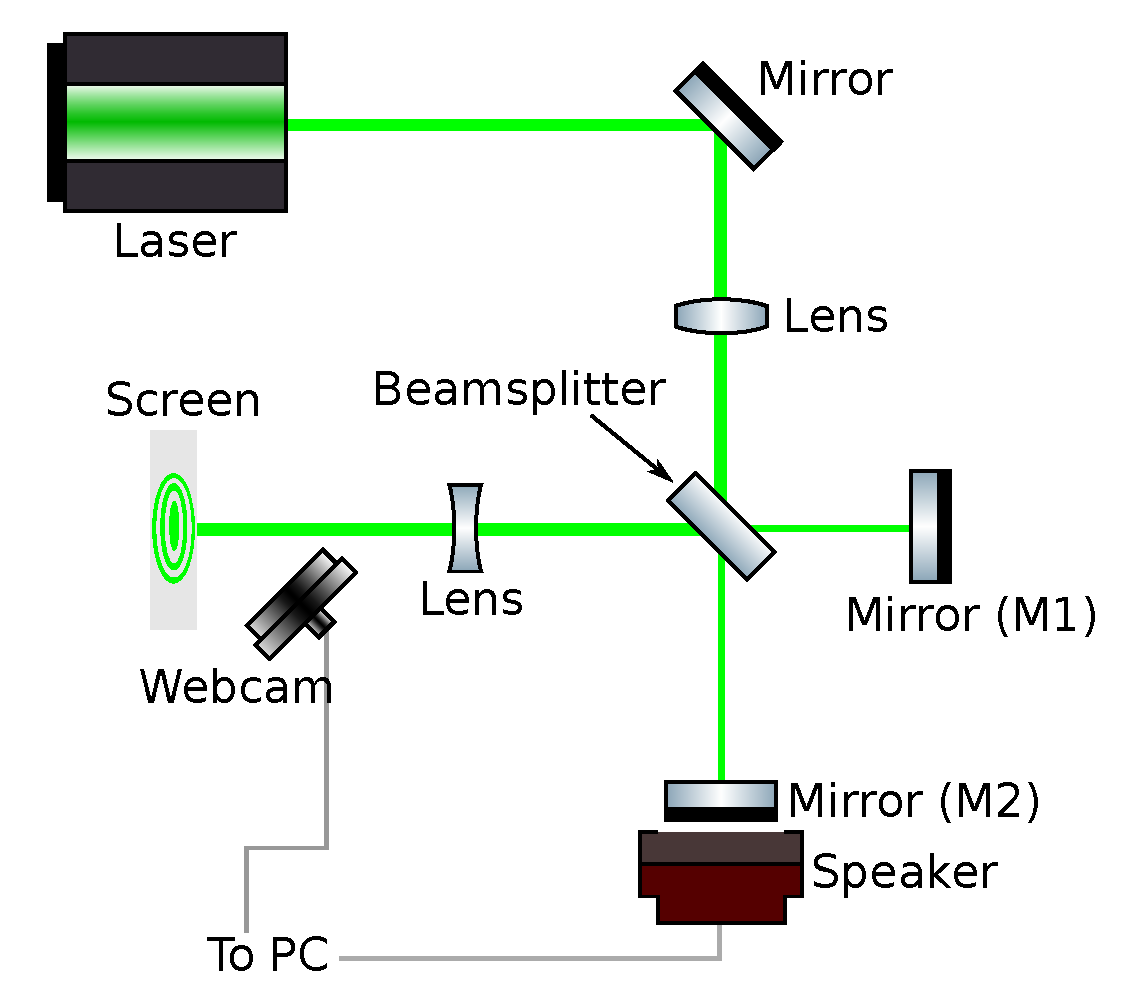
\includegraphics[width=0.5\textwidth]{figures/ifo_schematic_webcam_edit.pdf}
	\caption{\label{fig:ifo_schematic_webcam}
Schematic of the table-top Michelson interferometer. 
The output of a Class 2 $532\,{\rm nm}$ laser (top-left) is reflected from a mirror at a right angle. The beam then passes through a converging lens (focal length: $125.0\,{\rm mm}$) before reaching the beamsplitter which reflects approximately $50\%$ of the beam and transmits the remaining $\sim50\%$.
The split beams are reflected from mirrors (M1 and M2) at the ends of the interferometer arms and recombine at the beamsplitter. 
The output interference pattern is enlarged using a diverging lens (focal length: $-25.0\,{\rm mm}$), projected onto a screen, and recorded using a commercial webcam connected to a computer (PC). 
A speaker fixed to the back of M2 is used to inject audio signals from the PC into the interferometer.
    }
\end{figure}


The optical configuration of the Michelson interferometer used in this work is shown in Fig.~\ref{fig:ifo_schematic_webcam}.
It is assembled on a $450 \times 450 \,{\rm mm} $ optical breadboard and uses a green laser with peak emission at a wavelength of $532\,{\rm nm}$.
The output of the laser is first reflected by a mirror which turns the beam $90^{\circ}$ (to save space on the optical breadboard and to have greater control of the alignment of the interferometer).
After passing through a converging (plano-convex) lens with focal length $125.0\,{\rm mm}$, the laser beam is incident on a beamsplitter, which reflects half of the light towards mirror 1 (M1) and transmits the other half to mirror 2 (M2). 
A $0.5\,{\rm W}$ speaker is fixed to the back of M2 using commercial adhesive putty and serves as a controllable source of vibrations. 
This speaker is one of a pair of commercial, USB-powered speakers, fed by a $3.5\,{\rm mm}$ jack and driven by a computer (PC). 
The other speaker in the pair is kept face-down and as far away from the interferometer as possible to prevent it from acting as a second source.
The beams are reflected by mirrors M1 and M2, located at the end of $\sim 7.5\,{\rm cm}$ and $\sim 10.0\,{\rm cm}$ long arms.
The beams recombine at the beamsplitter and produce an interference pattern that is then enlarged using a diverging (bi-concave) lens of focal length $-25.0\,{\rm mm}$, and projected onto a screen.
The interference pattern, as shown by the photograph in Fig.~\ref{fig:interference_pattern}, is a set of concentric light and dark rings (fringes). 
A change in the relative length of the arms causes these rings to move radially inwards or outwards.
The intensity timeseries is recorded by either a webcam (in Sections~\ref{sec:single_tone} and~\ref{sec:viterbi_wandering}) or a photodiode, which offers a higher sampling rate suitable for capturing more complex audio (in Section~\ref{sec:optical_microphone}).
Further design details for Michelson interferometers can be found in Ref.~\cite{TTExhibit:2021}.



\begin{figure}
 \begin{center}
  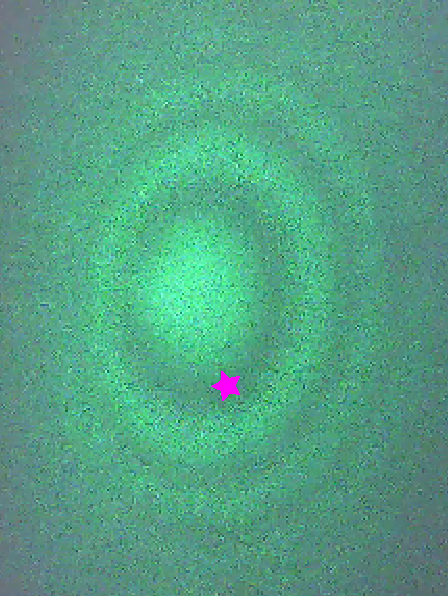
\includegraphics[width=0.35\textwidth, angle=-90]{figures/webcam_still0_star.pdf}
 \end{center}
 \caption{\label{fig:interference_pattern}
The interference pattern produced by the table-top Michelson interferometer.
This image was taken with the webcam aligned off the beam axis. 
The pink star indicates the point where the intensity timeseries measurements were taken.
The central bright fringe of the interference pattern is approximately $5\,{\rm mm}$ in diameter. 
}
\end{figure}

The motion of the interference fringes follows the motion of M2, and therefore of the speaker.
The amplitude of these motions is given by a transfer function that accounts for the coupling and resonance of the speaker-mirror system.
If the relative change in the length of the arms is kept small enough, then the intensity of the interference pattern at any point on the screen oscillates at the same frequency as the injected audio.
For larger relative length changes, multiple fringes will pass through the detection point during a single speaker oscillation, raising the measured frequency artificially. 
As such, any motion of the fringes must be kept small by playing the sound softly through the speaker.
Even without over-counting, large fringe motions display a nonlinear relation between the intensity fluctuations and injected audio, leading to troublesome---but physically interesting---phenomena like frequency doubling.



\end{document}
